\chapter[\Moha, a Silent Protest Behind the Viral Internet Meme]{{\sc M\'o-h\'a}, a Silent Protest Behind the Viral Internet Meme}\label{case}

\section{The culture background before the early age of Chinese digital era}
\dcap{A}{t the} National Conference of Publicity Ministers held on 10th January 2001, the then-president of the People's Republic of China (\prc) and General secretary of the Communist Party of China (\cpc) Jiang Zemin gave a speech, emphasizing that
\begin{quote}
	The publicity on the Internet should be paid particular attention, we should actively develop, sufficiently use, carefully manage the Internet publicity, make good use of its advantage and avoid its disadvantage, strengthen the impact and ``fighting capacity'' of the Internet publicity, make it a new battle field of political and ideological work\footnote{``Ideological work'' is a political term that commonly used in China, refer to activities and education that on behalf of certain social class or political groups, in order to achieve certain political objective, exerting ideological influence on people, and guide people's behavior on purpose. The term is likely translated from Russian word {\selectlanguage{russian}идеологическая работа} from the Soviet Union \citep{__2008-1}.} and a new medium of international publicity\footnote{Translated from Chinese by the author.}. \citep{__2001}
\end{quote}

As the so called core of the third generation of Chinese leadership, Jiang was facing a totally different picture of the country compared to his predecessors. He was nominated as the president unexpectedly in 1989, after the largest political protest referred as '89 Democracy Movement, including the 1989 Tiananmen Square protests and series of protest and demonstration through the country appealing for liberalization, freedom of the press, and re-evaluate the recently dead former president Hu Yaobang who was blamed within the \cpc\ for encouraging democracy and freedom, to replace his predecessor Zhao Ziyang, who was purged for his sympathize attitude to protesters. During the movement, Jiang as the then-mayor of Shanghai, successfully put down the protest by 1.\ appeasing protesters by direct informal communicate;\marginnote{See appendix \vref{timeline} for a more detailed timeline.} 2.\ employing police to guard main streets, ensure the order of regular operation of the city not affected; 3.\ putting pressure on the publisher of the newspaper \textit{World Economic Herald}, which published article supporting the movement and criticized the attitude of government \citep{kuhn_man_2005}.

Jiang's reaction to the protest to an extent represent his political position in his entire career, and a series of policies initiated during his presidency that influence the development direction of the country. One major reason of the '89 Democracy Movement is the Economic Reform initiated by Deng Xiaoping that introduced market economy, privatization, and foreign trade. The policy not only brought in western commodities, but also culture, knowledge, and here more important, political ideologies. Figure \ref{fig:westbook} shows the amounts of published philosophy literatures between 1980--1989, it is clear that the number was increasing and reached its peak at late 1987, then dropped to a very low point in 1989, i.e.\ when the '89 Democracy Movement occurred. Many publishing houses, especially university presses were formed the catastrophe of the Cultural Revolution and the launch of Economic Reform policy. In the period the western theories of democracy and freedom were extremely attractive for people in China, and apparently were learnt with passion \citep{__2011}.
\begin{figure}[!htbp]
	\centering
	\begin{tikzpicture}
  \begin{axis}[
  ybar,
  ymin=0,
  ymax=70,
  width=\textwidth,
  height=3in,
  grid=both,
  label style={font=\footnotesize},
  ytick distance=10,
  xtick distance=1,
  x tick label style={/pgf/number format/.cd, fixed,precision=0, set thousands separator={}},
  xlabel=year,
  ylabel=amount]
    \addplot[black,fill=white] table [x=year, y=amount, col sep=comma] {data/westbook.csv};
  \end{axis}
\end{tikzpicture}

	\caption[Amounts of translated western philosophy literatures, 1980--1989]{Amounts of translated western philosophy literatures, 1980--1989, reproduced from \citet{__2011}.}
	\label{fig:westbook}
\end{figure}

Except of the experience of ``fixing'' the citizens demonstration, Jiang also have a rich overseas study background---he used to work and study in Russian and Romania, and always keen to learn foreign languages. He was familiar with western context and its politics, however he used these knowledge in his own ways: on one hand, he catched the world's background of economic growth and promoted market economy, achieved a rapid economical development in China during his tenure, on the other hand, based on his knowledge of domestic and overseas citizen political activities, he introduced a series of policies to avoid all the ``unstable''  factors, and to make use of media, culture, and education to consolidate the domination of the government and authorites and to conduct their policies \citep{kuhn_man_2005,__2004}.

\section{The Internet censorship and the Great Firewall}

As \marginnote{{\tt "Ueber die Grosse Mauer erreichen wir alle Ecken der Welt"}\\\noindent{\tt "Across the Great Wall we can reach every corner in the world"}\\\noindent\citep{wang_first_1987}}a new and powerful media, Internet drew the attention of the government soon after it went popular. The first use of Internet in China can be tracked back to 1987 \citep{wang_first_1987,shrum_origin_2007}. In 1994, after test and building of infrastructure, China has been officially recognized able to access to Internet. In 1996, the China Golden Bridge Network opened a circuit to the \smallcaps{USA}, and started to provide service to individuals \citep{cernic_evolution_2001}.
\begin{figure*}[!htbp]
	\centering
	\begin{tikzpicture}[baseline]
  \begin{axis}[
  ymin=0,
  xmin=1997,
  xmax=2016,
  width=.6\textwidth,
  height=3in,
  yticklabel pos=upper,
  ytick distance=500,
  grid=both,
  label style={font=\footnotesize},
  x tick label style={/pgf/number format/.cd, fixed,precision=0, set thousands separator={}},
  legend style={legend pos=north west,font=\footnotesize},
  legend cell align=left,
  xlabel=year,
  ylabel=number of Internet users (millions)]
    \addplot[color=black, mark=square] table [x=year, y=china, col sep=comma] {data/internetuse.csv};\addlegendentry{China}
    \addplot[color=black, mark=triangle] table [x=year, y=world, col sep=comma] {data/internetuse.csv};\addlegendentry{worldwide}
  \end{axis}
\end{tikzpicture}
\begin{tikzpicture}[baseline]
  \begin{axis}[
  ymin=0,
  xmin=1997,
  xmax=2005,
  width=.4\textwidth,
  height=3in,
  yticklabel style={
        /pgf/number format/fixed,
        /pgf/number format/precision=5},
  %ytick distance=500,
  grid=both,
  label style={font=\footnotesize},
  x tick label style={/pgf/number format/.cd, fixed,precision=0, set thousands separator={}},
  legend style={legend pos=north west,font=\footnotesize},
  legend cell align=left,]
    \addplot[color=black, mark=square] table [x=year, y=china, col sep=comma] {data/internetuse.csv};\addlegendentry{China (zoomed in)}
    %\addplot[color=black, mark=triangle] table [x=year, y=world, col sep=comma] {data/internetuse.csv};\addlegendentry{worldwide}
  \end{axis}
\end{tikzpicture}


	\caption[Numbers of Internet users in China, 1997-2016]{Numbers of Internet users in China and worldwide, 1997-2016, Source: \citet{cnnic__2016}, and \citet{internet_live_stats_internet_2016}, which was estimated based on the data from International Telecommunication Union, World Bank, and United Nations Population Division.}
	\label{fig:internetchina}
\end{figure*}
After the introduction of Internet, the population of Internet users experienced a rapid increase, along with the global trend, until 2000 it doubled each year (see figure \vref{fig:internetchina}), and reached 53.2\% of the national total population at the end of 2016 \citep{cnnic__2016}.

The state's realization of supervising the information on the Internet was prompt. In 1996, the Ministry of Posts and Telecommunications (\mpt)\footnote{The predecessor of the current Ministry of Industry and Information Technology (\miit).} issued the \textit{Regulations of China on Administration of the Chinese Public Internet Connection to the International network}\footnote{\citet{__1996}, title and quotation translated by the author.}, mentioned that:
\begin{quote}
	\begin{description}[font=\rm]
		\item[\smallcaps{article 10}] Any organization by the author or individual must not use Internet to engage in criminal activity that harm national security or cause leak of state secret; must not use the international network to read, copy, produce, or spread information that harm national security, disorder the social order, or is obscene or pornographc.
		\item[\smallcaps{article 12}] Any individual or organizational Internet user, or Internet service provider must cooperate with relevant national department to supervise and examine the information security of international network, and provide material and convenience when necessary.
	\end{description}
\end{quote}
It is worth noting that, from this very early point, the \mpt\ already started to emphasize its right to collect information from Internet users and Internet service provider (\isp), and make distinction between domestic network and ``international network''.

Early in 1996,\marginnote{``While American and European governments have to legislate themselves the power to control the Internet, this is the default position for the Chinese government, and therefore constitutes one of the defining features of online China. The Internet, and by extension online China, are `government allowed'.''\\\noindent\citep{herold_noise_2011}}\ according to \citet{barme_great_1997}, the Public Security Bureau (\psb) already started to log the personal information of Internet users and filter the ``harmful'' websites by both administrative and technical means: individuals applying for Internet access have to provide \smallcaps{id}s, personal information including address, work place etc., and sign the \textit{Net Access Responsibility Agreement} which includes an agreement to not ``read, copy, produce, or spread information that harm national security, disorder the social order, or is obscene or pornographic''; and \isp s had been running keywords-based filtering to block websites that contain political sensitive materials, which is relatively easy since all international connections have to be made through state owned \isp s, and the access routes are owned and controlled by the government, from which individuals and organizations only have the right to rent bandwidth.  \citep{herold_escaping_2012,herold_noise_2011,barme_great_1997}. A study conducted by \citet{zhang_behind_2006} directly with the policy makers shows that the new technologies not only caused new policies and ``game plan'', but also reshuffled of policy making process, the ``frame of negotiation'' \citep[p.~147]{price_media_2002}. The main responsibility of managing the media and information had been shifted from directly the \cpc, to the committee China Internet Network Information Center (\cnnic) Steering Committee formed in 1997, which consisted of both scholars and government officers \citep[p.~281]{zhang_behind_2006}. The interviewed authorities states the ``two-hand strategy'' of policy making, that ``promoting development of the [I]nternet, [policy makers] have to supervise and regulate the content'', the government was intended to make use of the benefit of economical growth and information exchange by encouraging it, but meanwhile keep away the unfavorable materials \citep{zhang_behind_2006}.

The major instrument that the Chinese government currently use, the \gfw\footnote{This term was likely be coined by \citet{barme_great_1997} in the \textit{WIRED} magazine article, later was commonly accepted but never be referred nor admitted \textit{per se} by the Chinese official.}, started its development in 1998 (although the term was used \textit{avant la lettre} a year before as a metaphor to the general idea of Chinese Internet censorship), and lunched at 2003 according to the leading designer of the \gfw\ Fang Binxing \citep{global_times_great_2011}. So far, the major techniques of the \gfw\ include \smallcaps{ip} blocking and \smallcaps{dns} tampering and hijacking, which blocks sensitive blacklisted websites e.g.\ Google or specific service on specific servers directly; the deep packet inspection and keyword filtering, which could censor the real time Internet traffic and block the webpage or service that contains specific keyword, and recently even active attack \citep{xu_deconstructing_2016,yuen_becoming_2015,perlroth_chinese_2015}.

However, a more powerful way is the self-censorship, where the ``the general sense that you are under surveillance acts as a disincentive. The key to controlling the Net in China is in managing people, and this is a process that begins the moment you purchase a modem'' \citep{barme_great_1997}. The policy makers see the act of censoring not only as a means of regulation, but a kind of education, through which website managers and users would regulate what they post on the Internet by themselves \citep{zhang_behind_2006}. In 2015, after the code hosting website GitHub have been DDoS attacked likely by Chinese government\footnote{The Ministry of Foreign Affairs of the \prc\ (\mfa) did not admit nor deny the government initiate the attack, however some research shows that the attack has the similar Internet characteristics as the \gfw, therefore it is mostly believed that this is the action of the Chinese government \citep{brandom_last_2015,perlroth_chinese_2015}.}, many Chinese users of GitHub rise the argument that users should regulate themselves not post political sensitive materials on the site, since the government may ban the site for these materials and all ``innocent'' users would be affected \citep{__????-16}. Domain websites in China were asked to sign a pledge in 2002, in which they promised to not produce and spread pernicious information on their website, remove sensitive materials (otherwise relevant staff could face expulsion), and to monitor foreign-based websites \citep{the_guardian_chinese_2002}. The \usa\ Internet company Yahoo! also signed the pledge, and on 2006 it was criticized in west for providing information of online activities of user to the Chinese government, and caused the arrest of a pro-democracy journalist Shi Tao \citep{the_associated_press_yahoo_2007}. The standard of the self-censorship became more strict, in a conference at 2016, the Cyberspace Administration of China (\cac) asked domain websites to verify the body of responsibility for all posted information, control the sources of news posts (commercial websites were no longer allowed to produce news posts by themselves), and be responsible 24$\times$7 in the case of emergency. Earlier this year many originate news sections of major websites were shut down for posting mistaken information related to the president Xi Jinping \citep{_8_2016}.

By conducting the sense of insecurity, through privatized enforcement (letting \isp s to take the responsibility of filtering contents) and surveillance, the state actually make the virtual space a Panopticon, that the exact choice of censored words never been told or explained to the users, but was given the sense that certain content are generally \textit{known} to exist \citep{vuori_lexicon_2015,boyle_foucault_1997}. The research conducted by \citet{vuori_lexicon_2015} concerning keyword filtering systems on Chinese social networks shows that almost 16.26\% of all messages posted on the largest Chinese tweeter-like microblog service Weibo are deleted over time, especially those are ``politically sensitive'' or potentially lead to ``collective action'' one third of censored keywords are related to names of leading members of the \cpc. According to \citet{foucault_security_2007}, through the technique of surveillance and correction, discipline is operated in the way that people do things spontaneously and without knowing the influences on their behaviour. While covered by the means of technologies, the manipulation of information by sovereign is usually accepted by the users as they are without noticing its political origins. The censorship in Chinese Internet is not intended to actually stop people seeing the political related contents, at least the names of party leaders are being repeatedly mentioned on official medias all the time, but to make the free communication about the ``leading personalities'' freely by simply referring their names more difficult, and thus ``hinders their ability to form shared critical opinions on them and their policies'' \citep[p.~413]{vuori_lexicon_2015}.

\section{The viral subculture of toad-worshiping}\label{sec:moha}

If one is using Chinese social networks in recent years, one would occasionally see curated stickers, pictures, videos, and quotes from the ex-president (from 1989 to 2002) Jiang Zemin. The culture phenomena referred as \moha\ (膜蛤, literally toad worship) went increasing popular especially after Xi Jinping became the current president in 2012.
\begin{marginfigure}
	
\includegraphics[width=\textwidth]{mohasample1.jpg}
	\caption[A sample of meme picture based on the portrait of Jiang Zemin]{A sample of meme picture based on the portrait of Jiang Zemin.}
	\label{fig:mohasample1}
\end{marginfigure}

In the term ``\moha'', Jiang has been assimilated to a toad (蛤蟆, \textit{h\'a-ma}) for his signature appearance: oversized black frame glasses, broad mouth, and high-waisted pants \citep{_jiang_2016}. The metaphor is first used by Falun Gong (also known as Falun Dafa) as an insulting nickname of Jiang. Falun Gong is a spiritual practice group that has been categorized as ``heretical organization'' by the Chinese government and banned in mainland China since late 1999. The group has held a radical and hostile attitude toward the \cpc\ and the then-party leader Jiang. In early 2000s, around ten years before \moha\ eventually became popular, the Falun Gong created, although it went against their original intention, the basic ground of the subculture, and funded one of the most popular Internet censorship circumvention software at that time, Freegate, that allows Internet users in mainland China to bypass the \gfw\ and accessing the blocked content. Freegate features Epoch Times\footnote[][-.7cm]{The website has been hosted in \usa\ and banned in Chinese Internet since the beginning.} as its homepage. The website contains a lot of information that against \cpc\ and Jiang himself, lots of which are travesty (see figure \vref{fig:flg1}) and crudely made folk stories e.g.\ portraying Jiang as a sprite of toad.
\begin{figure}[!htbp]
	\centering
	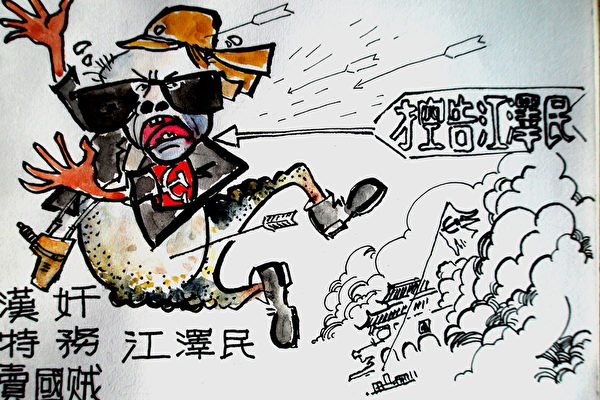
\includegraphics[width=\textwidth]{flg1.jpg}
	\caption[A cartoon posted on the Falun Gong sponsored news website Epoch Times]{A cartoon posted on the Falun Gong sponsored news website Epoch Times. Left text: traitor of China/foreign spy/quisling Jiang Zemin; right: accuse Jiang Zemin. Source: \citet{__????-162}.}
	\label{fig:flg1}
\end{figure}
They also posted large amount of video materials related to Jiang, especially those with his negative figures. Most users of Freegate at that time are usually high-educated (accessing most blocked websites requires English reading skill, and basic computer skills) and politically pro-liberalization (bypassing the \gfw\ is politically ``dangerous'' in the context of \cpc\ conservatives). However, these effort Falun Gong made did not make big influence on most Chinese Internet users, even those who bypassed the \gfw: most of them would not believe the exaggerated stories, at most amused by the funny behavior of the president in those materials.

In this phenomena, the funniness of Jiang himself played an important role for its viral spreading. His rich overseas experience, interests in art and foreign languages, and his exhibitionist, humorous nature made his very different figure compared to other political leaders in China. In many of his video footages, mostly available on non-Chinese websites such as YouTube and treated as treasures by toad-worshippers, he plays music, sometimes with local instruments during overseas visit, dances, and sings in public occasions. During his 1993 visit to \usa, he happily invited Bill Clinton to play saxophone with him \citep{kuhn_man_2005}. In his interview with Mike Wallace, he answered Wallace's harsh questions about the accusation of dictatorship and '89 Democracy Movement calmly with smile, sometimes even sidestepping the translator and answering directly in English.

The major materials used to produce the \moha\ related memes, derivative works, and parodies are three videos (will be referred as \smallcaps{video 1}, \smallcaps{2}, and \smallcaps{3} afterward):
\begin{enumerate}
	\item The\marginnote{\smallcaps{video 1} is available at \url{https://youtu.be/NsGbhDVFxQw}} video of Jiang's angry response to Hong Kong journalists \citep{pbs_nc_2000}. In a media session, Jiang was asked whether Beijing would endorse the then-chief executive Tung Chee-hwa for a second term. After which he got angry,  then angrily chastised the journalist for around three minutes \citep{landler_leader_2000}.
	\item The aforementioned\marginnote{\smallcaps{video 2} is available at \url{https://youtu.be/3w4dy-VZjBw}} video of Jiang's interview with Mike \citet{wallace_president_2000}.
	\item The video\marginnote{\smallcaps{video 3} is avaliable at \url {https://youtu.be/lsZjnO4NwYw}} of Jiang's revisit of China United Engineering Corporation on 2009. Jiang used to work in the predecessor of this corporation as a engineer. In the video he summarized his experience of being summoned to Beijing and unexpectedly became the president, and his ``three achievements'' during his term. While receiving a gift given by the staff, he said ``This book you give me\ldots\ \textit{Excited!}\footnote{The word was said in English.}''.
\end{enumerate}
Almost every sentence in \smallcaps{video 1} (a more detailed analyse of the creation of memes out of the video is presented in appendix \vref{script}), many screenshot from \smallcaps{video 2}, and lots of sentence from \smallcaps{video 3} especially a piece of poem Jiang read during his speech and the ``excited!'' he said in English became the most popular quotes in the \moha\ subculture. Figure \vref{fig:keywords} shows the trend of search interest from China. Five keywords are selected:
\begin{figure*}[ht]
	\centering
	\begin{tikzpicture}[baseline]
  \begin{axis}[
  ymin=0,
  xmin=2004-01-01,
  xmax=2017-08-01,
  ymax=100,
  width=\textwidth,
  height=3in,
  grid=both,
  y filter/.expression={y==0 ? nan : y},
  label style={font=\footnotesize},
  x tick label style={rotate=45,/pgf/number format/.cd, fixed,precision=0, set thousands separator={}},
  legend style={legend pos=north west,font=\footnotesize},
  legend cell align=left,
  xlabel=year,
  date coordinates in=x,
  date ZERO=2004-01-01,
  xticklabel=\year.\month,
  ylabel=popularity,
  xtick = {
  {2004-01-01},
  {2004-07-01},
  {2005-01-01},
  {2005-07-01},
  {2006-01-01},
  {2006-07-01},
  {2007-01-01},
  {2007-07-01},
  {2008-01-01},
  {2008-07-01},
  {2009-01-01},
  {2009-07-01},
  {2010-01-01},
  {2010-07-01},
  {2011-01-01},
  {2011-07-01},
  {2012-01-01},
  {2012-07-01},
  {2013-01-01},
  {2013-07-01},
  {2014-01-01},
  {2014-07-01},
  {2015-01-01},
  {2015-07-01},
  {2016-01-01},
  {2016-07-01},
  {2017-01-01},
  {2017-07-01}
  }]
    \addplot[only marks, mark=pentagon] table [x=month, y=popularity, col sep=comma] {data/excited.csv};\addlegendentry{excited}
    \addplot[only marks, mark=diamond] table [x=month, y=popularity, col sep=comma] {data/gouliguo.csv};\addlegendentry{苟利国家生死以}
    \addplot[only marks, mark=o] table [x=month, y=popularity, col sep=comma] {data/hah.csv};\addlegendentry{蛤蛤}
    \addplot[only marks, mark=+] table [x=month, y=popularity, col sep=comma] {data/hkj.csv};\addlegendentry{香港记者}
    \addplot[only marks, mark=x] table [x=month, y=popularity, col sep=comma] {data/tanxiao.csv};\addlegendentry{谈笑风生}
    \addplot[only marks, mark=star] table [x=month, y=popularity, col sep=comma] {data/xum.csv};\addlegendentry{续命}
  \end{axis}
\end{tikzpicture}


	\caption[The search interest over time of \moha\ related keywords from China, from Jan 2014 to Jul 2017]{The search interest over time of \moha\ related keywords from China, from Jan 2014 to Jul 2017. A value of 100 is the peak popularity for the term, and a value of \textit{x} represent the keywords' popularity is \textit{x}\% of its peak value. Source: \citet{google_google_????}. Sudden zero points are considered as error and have been ignored in the plot.}
	\label{fig:keywords}
\end{figure*}
\begin{description}
	\item[Excited] This is the word Jiang said during the visit from \smallcaps{video 3}. It is also one of the most commonly referred word in the \moha\ subculture, it is short, easy to remember and is flexible to be used in varies way. It is noticeable that even \textit{excited} is a common English word that not only used as a meme, its search interest also experienced the similar increase along with the other exclusively \moha\ related keywords.
	\item[苟利国家生死以 (Were it to benefit my country I would lay down my life)] This is the first of two sentence of the poem Jiang recited in \smallcaps{video 3} \footnote{苟利国家生死以,岂因祸福避趋之。(\textit{Were it to benefit my country I would lay down my life; What then is risk to me?}, translation from \citealp{central_compilation__translation_bureau_2015_2015}). It was originally from a poem written in 1842 by Lin Zexu.}. He used this to show his determination when he was nominated to be the president. This represent Jiang's allusive personality, and was also frequently quoted by toad-worshippers, sometimes as it is, sometimes abbreviated form such as using the first character 苟 (\textit{g\v ou}), or initial of both sentence 苟岂 (\textit{g\v ou q\v{\i}}), their homophonies, etc.
	\item[蛤蛤 (h\'a-h\'a, toad)] This is the nickname of Jiang given by toad-worshippers. 蛤 (\textit{h\'a}) Literally means toad or clam, but if used repeatedly as \textit{h\'a-h\'a}, this word can be considered exclusively used by the \moha\ subculture, therefore it is chosen to indicate the popularity of the subculture.
	\item[香港记者 (Hong Kong journalist)] This term is from \smallcaps{video 2}, referred to the Hong Kong journalist who was angrily chastised by Jiang. This term is not only used by toad-worshippers, but also used in in everyday conversation, it could be clearly seen from figure \vref{fig:keywords} that even the term also been used elsewhere, its search interest still increased significantly after 2014.
	\item[谈笑风生 (talk cheerfully and smoothly)] This is an idiom Jiang used in \smallcaps{video 1} to referred to his interview with Mike Wallace.
	\begin{marginfigure}
		\begin{tikzpicture}[baseline]
  \begin{axis}[
  ymin=0,
  xmin=2013-01-01,
  xmax=2017-08-01,
  ymax=100,
  width=\textwidth,
  height=2in,
  grid=both,
  y filter/.expression={y==0 ? nan : y},
  label style={font=\footnotesize},
  x tick label style={rotate=45,/pgf/number format/.cd, fixed,precision=0, set thousands separator={}},
  legend style={legend pos=north west,font=\footnotesize},
  legend cell align=left,
  xlabel=year,
  date coordinates in=x,
  date ZERO=2004-01-01,
  xticklabel=\year.\month,
  ylabel=popularity,
  xtick = {
  {2013-01-01},
  {2013-07-01},
  {2014-01-01},
  {2014-07-01},
  {2015-01-01},
  {2015-07-01},
  {2016-01-01},
  {2016-07-01},
  {2017-01-01},
  {2017-07-01}
  }]
    \addplot[color=black, mark=star] table [x=month, y=popularity, col sep=comma] {data/xum.csv};\addlegendentry{续命}
  \end{axis}
\end{tikzpicture}


		\caption[The search interest over time of the keyword ``续命'' around Aug 2015]{The search interest over time of the keyword ``续命'' around Aug 2015. Source: \citet{google_google_????}. Sudden zero points are considered as error and have been ignored in the plot.}
		\label{fig:keywordsz}
	\end{marginfigure}
	\item[续命 (life extension)] This is a term used frequently in the \moha\ subculture, suggesting that every time someone posts, acts, or reacts at something related to Jiang or relevant memes, Jiang's life would be extended for one second, and eventually would make him immortal. The origin of this action was is likely based on the 2011 news that mistakenly reported Jiang had died \citep{blanchard_china_2011,bbc_hong_2011}, and some similar rumors occasionally popped up afterward. Some toad-worshippers would post ``+1s'' or similar phrases when they see some \moha\ related or triggered content, acknowledging that his life has been extended. Figure \vref{fig:keywordsz} shows a rapid growth of the activity of this term around 17th Aug, which is Jiang's birthday, this was a recent climax of toad-worshippers' activity.
\end{description}

\section{How implicit political expression hijack the ordinary language in the virtual space}
why are there an increasing number of people looking to extend an ex-president's life (even mockingly)? Why there were so many people exchanging gossip of a 90 years old politician, and calling themselves worshipper? Why those materials spread by Falun Gong to bring shame on Jiang, seemingly conversely draw people's affection? \citet[pp.~7--8]{shifman_introduction_2014} states that Internet memes can be defined as ``a \textit{group of digital items sharing common characteristics}\footnote{Emphasised as the original.} of content, form and/or stance'', that ``were created with awareness of each other'' and could be circulated and reproduced through Internet users.

As discussed in section \ref{sec:moha}, the subculture of \moha\ experienced a rapid expansion since 2014, before which almost all the materials of the related memes had already been circulated on the Internet for more than 10 years. As the memes use discourse as material that reflect the socioeconomic factors on communication, and ``only memes suited to their sociocultural environment spread successfully'' \citep{shifman_telegraphic_2014,johnson_mapping_2007}, the reason of the emerging of \moha\ subculture clearly have some relation with the sociocultural environment around 2014. Although Chinese government has taken a series of actions to implement the Internet censorship and surveillance, however in 2000s, it was relatively easy to bypass them by simply install softwares or using \vpn. The current president Xi Jinping came to power at 2012, since then the government has been formulating much tighter policies of culture and personal expressions. According to a 2013 regulation about real-name telephone system approved by \citet{miit__2013}, anyone in mainland China purchasing a mobile phone number have to provide a valid \smallcaps{id}s\footnote[][-2,5cm]{Compared with most western countries, although there are also certain kind of censoring, it is still easy to purchase anonymous mobile phone numbers that able to access to Internet, or hide the user identity (at least on the personal level) using services such as \vpn, Tor, etc. without trouble.}, and another regulation passed in 2015, stipulates that all \isp s should follow the principle of ``real-name in the background, optional in the foreground'' \citep{miit__2015}. Currently most mainstream Chinese \isp s require a valid mobile phone number to register, which means anyone living in China who post unfavoured content on the Internet could be trancked directly to the person. A proxy software developer, who has posted supportive opinion to the Occupy Central campaign\footnote{The campaign took place in Hong Kong, intended to protest to the \prc\ government to grant to the right for universal suffrage for Hong Kong citizens \citep{branigan_occupy_2014}. This campaign was recognized as an illegal Hong Kong independence activity and be denounce by the \prc\ and \cpc\ official \citep{_--_2014}.} on Twitter was arrested in 2014 for Crime of Picking Quarrels \& Provoking Troubles \citep{__????-17}. The first Law specifically about Internet \textit{Cybersecurity Law of the \prc} was passed in 2015, explicitly states that all \isp s must require users to provide their valid \smallcaps{id} when providing Internet accessing service, must cooperate with national security departments when necessary, must report to the national security departments when any illegal information was detected, and could cut down the Internet in certain area when urgent situation appears \citep{__waf}.

The discontent sentiment for Xi's restrictive attitude toward the Internet freedom is another major element in the \moha\ related memes. Figure \vref{fig:jiangxi} shows a pair of book covers of Jiang and Xi's biographies. The former is the actual cover of the book by \citet{kuhn_man_2005}, which takes a positive comment to Jiang's presidency, and has been banteringly praised within the toad-worshippers' group, while the latter is a fictive book cover that has been circulated on the Internet.
\begin{figure}[!htbp]
	\centering
	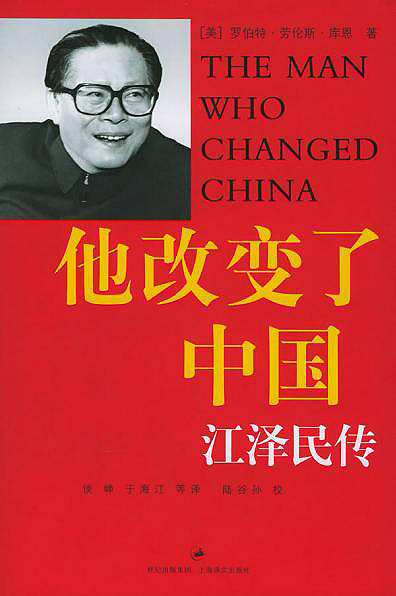
\includegraphics[width=.45\textwidth]{jiang.jpg}
	\hfill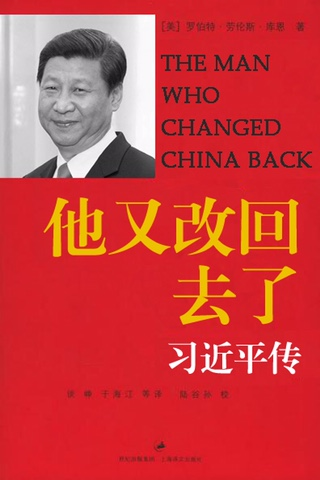
\includegraphics[width=.45\textwidth]{xi.jpg}
	\caption[Satiric fictive book cover of Xi Jinping's biography compared to the actual Jiang's]{Satiric fictive book cover of Xi Jinping's biography compared to the actual Jiang's. Left text: He changed China---A biography of Jiang Zemin; right: He then changed it back---A biography of Xi Jinping.}
	\label{fig:jiangxi}
\end{figure}
While the title of Jiang's biography \textit{The man who changed China} usually be understood as his positive impact on Chinese economic growth, and facilitate formal and informal international communication based on the economic reform policy initiated by Deng Xiaoping. The satiric title \textit{The man who changed China back} implies the unsatisfactory to Xi's policies of strengthen Internet and press censorship and the personality cult built by propaganda \citep{beech_chinas_2016}, and his changing to society back to the ``old society'', which in Chinese context often means feudal, totalitarian imperial society before the mid 20th century \citep{cohen_cultural_1993}. Ironically, both of the pictures were banned in the dominating\footnote{More than two thirds of handset owners use it regularly in 2017 \citep{mcnair_wechat_2017}.} Chinese instant message application WeChat, which displayed as sent in the sender's side but won't be received\footnote{Tested by the author on 3rd July 2017.}. In mid 2017, the cartoon character Winnie-the-Pooh was censored in Chinese social networks because its similar appearance to Xi \citep[see figure \vref{fig:winnie}]{hernandez_winnie--pooh_2017}.

Along with the increasing censorship since 2012, while \textit{talking about politics} or even simply party leaders has been becoming dangerous, people started to search for new way of political expressions. \citet{scott_behind_1990} describes the mechanism of ``public transcripts'' that happens in the public domains that subordinates (or those take the weak side of the power relationship) act with subordination to the dominant power, ``offer a performance of deference and consent while attempting to discern, to read, the real intentions and mood of the potentially threatening powerholder''. However the implied intention that challenging the powerholders, with the coded information that only who with awareness or certain political position can understand, a kind of \textit{unobtrusive dissent} \citep{perry_studying_2007,esarey_political_2008,scott_behind_1990}. In the early 2000s, the materials released by Falun Gong were all explicitly pointed to Jiang himself, with his name and figures. Today, the terms and figures used by toad-worshippers are degraded more and more close to ordinary languages. ``苟'' (\textit{g\v ou}) is a common Chinese characters and usually means nothing if used by its own, however it became a kind of secret signal between toad-worshippers, when someone see an Jiang related content, or simply just want to draw attention of other toad-worshippers, he/she could just post this one single character and noticed toad-worshippers would follow and reply with other characters from the poem.
\begin{marginfigure}[-12cm]
	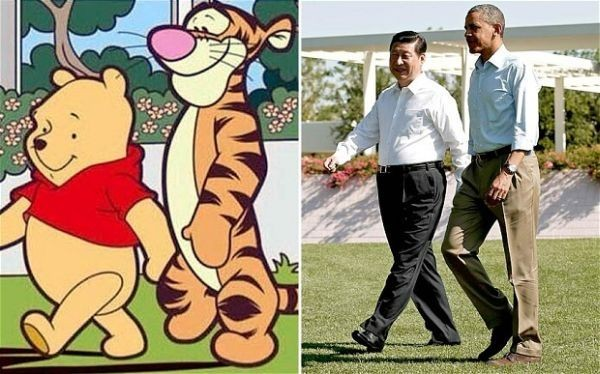
\includegraphics[width=\textwidth]{pooh.jpg}
	\caption[The picture that has been circulated on the Internet showing Xi Jinping and Barack Obama resemblance to Winnie-the-Pooh and Tigger]{The picture that has been circulated on the Internet showing Xi Jinping and Barack Obama resemblance to Winnie-the-Pooh and Tigger.
		\label{fig:winnie}}
\end{marginfigure}

\begin{figure}[!htbp]
	\centering
	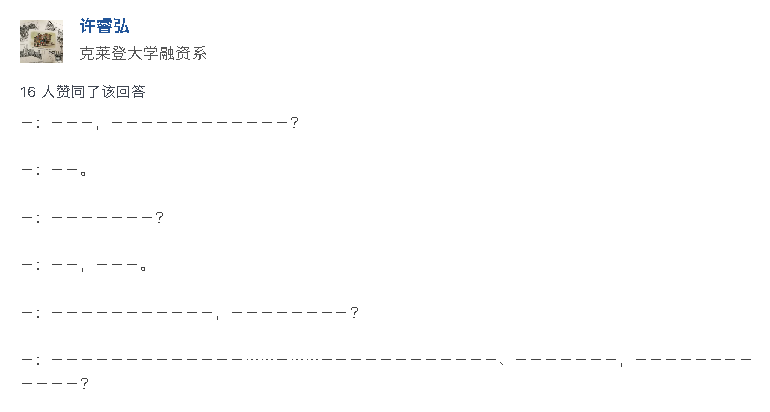
\includegraphics[width=\textwidth]{zhihu.pdf}
	\caption[An answer posted on Chinese question-and-answer website Zhihu implies script of the conversation in the video of Jiang Zemin angrily chastised the Hong Kong journalist]{An answer posted on Chinese question-and-answer website Zhihu implies script of the conversation in the video of Jiang Zemin angrily chastised the Hong Kong journalist, answering the question ``What story could you write if only using punctuation marks?''. Source: \url{https://www.zhihu.com/question/60370256}.}
	\label{fig:zhihu}
\end{figure}

Figure \vref{fig:zhihu} shows a typical implied \moha\ activity, that one of the users of the question-and-answer website Zhihu posted a long list of seemingly meaningless dashes and punctuation marks. They are actually the script from the conversation between Jiang Zemin and the Hong Kong journalist in \smallcaps{video 1}, with all texts been substituted by dashes.
\begin{figure}[!htbp]
	\centering
	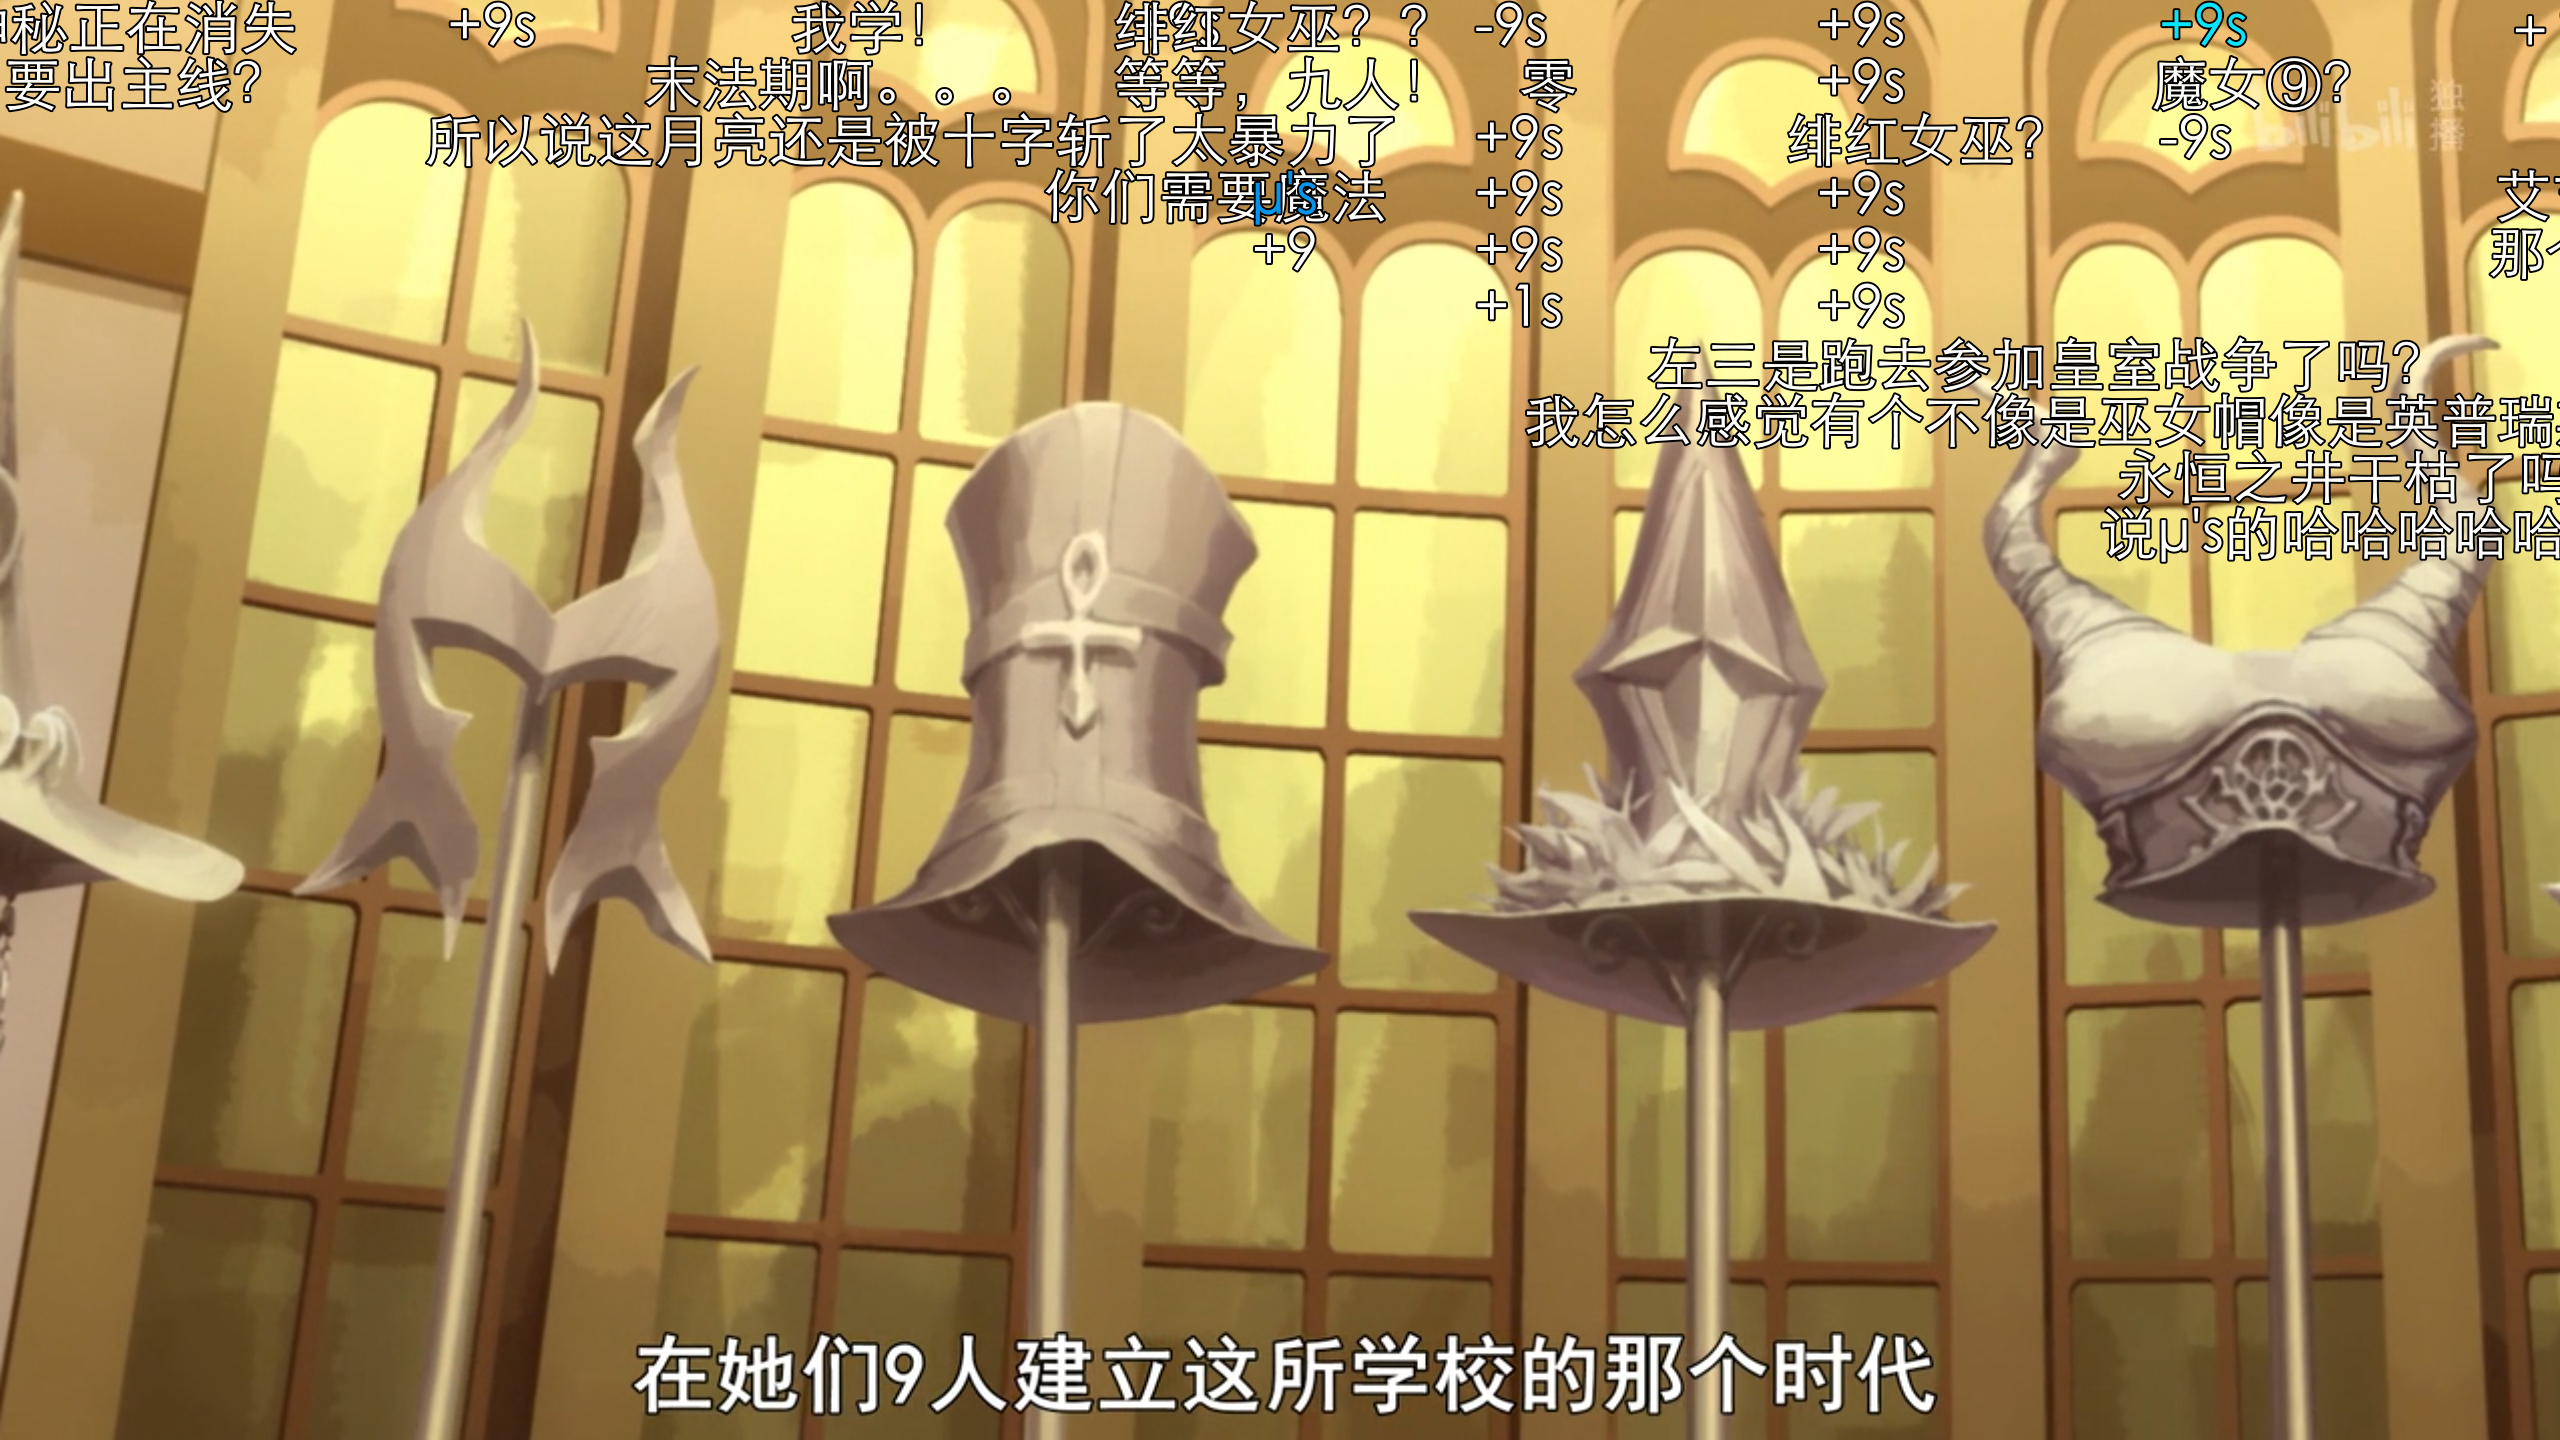
\includegraphics[width=\textwidth]{scnst.png}
	\caption[A screenshot from a Chinese bullet comment video website while audience posting ``life extension'' comments]{A screenshot from a Chinese bullet comment video website while audience posting ``life extension'' comments. Source: \url{https://bangumi.bilibili.com/anime/5788/play\# 101771}; The video: \citet{yoshinari_blue_2017}.}
	\label{fig:xmn}
\end{figure}
Figure \vref{fig:xmn} is another example, in a bullet comment video website Bilibili, when the line in the anime mentioned ``九长者'' (nine elders), audiences started posting comment such as ``+1s'' or ``+9s'' on the screen. ``Elder'' is the what Jiang had called himself during his chastise to the journalist: ``today I am not as a president, but an elder, to teach you some experience of life''. The content of the anime does not have any relation to Jiang, and the word has just been used normally, but the toad-worshippers were still be triggered, and hijacked the unrelated material as their own. To an extent, any language, images, or objects that contains or has any similarity to
\begin{enumerate*}
	\item quotes from Jiang, or any homophony of it, e.g.\ ``excited'', ``na\" ive'', etc.;
	\item Jiang's appearance: high waist pants, black frame glasses, or anything looks like them;
	\item any person or action that related to or had been mentioned by Jiang, e.g.\ Hong Kong journalists, ``running fast'', the university Jiang used to studied in (Shanghai Jiao Tong University), etc.;
	\item Any language or object that could be related to the \moha\ subculture itself, e.g.\ anything contains character ``膜'' (\textit{m\'o}: worship/ film/membrane), ``蛤'' (\textit{h\'a}: toad/frog/calm), ``extend'', ``one second'', etc.
\end{enumerate*}
\begin{marginfigure}
	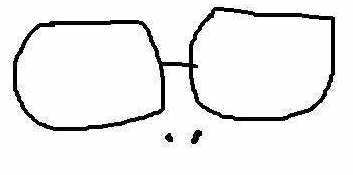
\includegraphics[width=\textwidth]{blm.jpeg}
	\caption[A sketch circulated on the Internet that implies Jiang by glasses and nostrils]{A sketch circulated on the Internet that implies Jiang by glasses and nostrils.}
	\label{fig:simplemo}
\end{marginfigure}

These actions, rather than expressing certain political opinion, is more like a kind of ritual. It is easy to remember and repeat, and is interesting and fun. Every time the \moha\ activity is triggered, whether intentional or by unrelated thing, a context is created that only those who share the knowledge of this subculture---not only know about Jiang, but know him in the way of \moha. Like the Soviet joke describe:
\begin{quote}
	A man is distributing leaflets in Red Square. He is stopped by a policeman, who confiscates them, only to discover that they are blank. ``What are you spreading? They are blank. Nothing is written!'' the surprised guardian of order exclaims. ``Why write?'' is the answer. ``Everybody knows\ldots'' \citep[p.~2]{przeworski_prologue_1991}
\end{quote}
Through the practice of these activities, a counter-discourse was built: \textit{talking about politics} is political, and being political itself is conceived as dangerous in contemporary China. By practicing \moha, toad-worshippers are talking (satirizing, making fun of) about the former top party leader, in a way that their the political critiques have been normalized to a extremely ordinary level that can hardly be censored, censoring single characters is nearly impossible, neither censoring everything with two ovals and two dots (see figure \vref{fig:simplemo}), or simply some dashes (figure \vref{fig:zhihu}). The ritual is a \textit{confirmation} between toad-worshippers. The joke of ``life extension'' could be seen as a calling, that what toad-worshippers actually want to extend is the time with loose policies for speech and political expressions, international communications, and rapid economic growth; and what Jiang's personal figure represents---art lover, can speak many foreign languages, humour (which has  extincted on the two successors of Jiang), and human emotions---he was a president that would chastise a journalist. By contrast, Xi Jinping has been criticized for his bad personal taste: in a speech given in 2014, he listed 112 artists by name without in one time without any detail and context \citep{__2015-3,chin_year_2015}. He also said on another conference that architects should avoid ``strange-looking buildings'' and encouraging patriotic art \citep{alyssa_abkowitz_xi_2014}. It is ironic that although the \gfw\ was actually initiated during Jiang's presidency, due to the technical resource and government's less knowledge to the Internet, compared with later yeas, the period of early 2000s was still the peirod that Chinese Internet users have most freedom.
